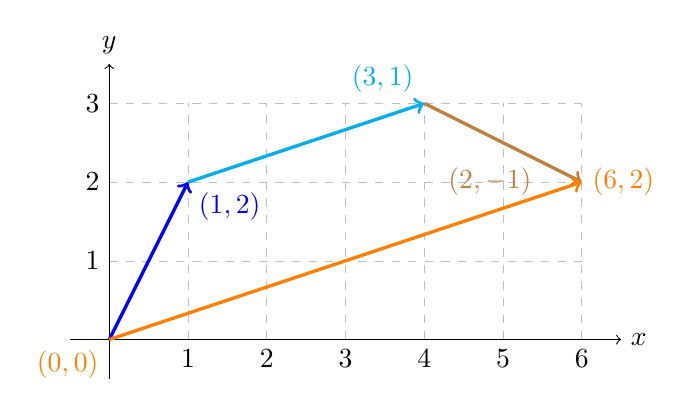
\begin{tikzpicture}
    \draw[step=1,help lines, dashed,lightgray] (0,0) grid (6,3);
    %draw axis value
    \foreach \x in {1,2,...,6}
        {%
            \draw (\x,0) -- (\x,0) node [below] {$\x$};
        }
    \foreach \y in {1,2,3}
        {%
            \draw (0,\y) -- (0,\y) node [left] {$\y$};
        }
    %draw lines
    \draw [->] (-0.5,0) -- (6.5,0) node[right]{$x$};
    \draw [->] (0,-0.5) -- (0,3.5) node[above]{$y$};
    \draw [->,blue,very thick] (0,0) -- (1,2) node[below right]{$(1,2)$};
    \draw [->,cyan,very thick] (1,2) -- (4,3) node[above left]{$(3,1)$};
    \draw [->,brown,very thick] (4,3) -- (6,2) node[left]{$(2,-1)\hspace{5mm}$};
    \draw [->,orange,very thick] node[below left]{$(0,0)$} (0,0) -- (6,2) node[right]{$(6,2)$};
\end{tikzpicture}
\captionof{figure}{{\footnotesize (1,2)+(3,1)+(2,-1)=(6,2)}}
\label{fig:vector-and-vector-operation-d8}
